\section{Networking Libraries}
\label{app:network-code}

\begin{figure}[t]
\begin{scriptsize}
\begin{lstlisting}
module BestEffortDelivery
  include DeliveryProtocol

  def state
    channel :pipe_chan,
      ['@dst', 'src', 'ident'], ['payload']
  end

  def initialize(host, port, opts)
    @addy = "#{host}:#{port}"
 end

  declare
  def snd
    pipe_chan <~ pipe_in
  end

  declare
  def done
    pipe_out <= pipe_in
  end
end
\end{lstlisting}
\centering
\vspace{-10pt}
\caption{Delivery modules.}
\label{fig:delivery-impl}
\end{scriptsize}
\vspace{-2pt}
\end{figure}


\begin{figure}[t]
\begin{scriptsize}
\begin{lstlisting}
module MulticastProtocol
  def state
    table :members, ['peer']
    interface input, :send_mcast, ['ident'], ['payload']
    interface output, :mcast_done, ['ident'], ['payload']
  end
end

module Multicast
  include MulticastProtocol
  include DeliveryProtocol

  declare
  def snd_mcast
    pipe_in <= join([send_mcast, members]).map do |s, m|
      [m.peer, @addy, s.ident, s.payload]
    end
  end

  declare
  def done_mcast
    # override me
    mcast_done <= pipe_out.map{|p| [p.ident, p.payload]}
  end
end
\end{lstlisting}
\centering
%%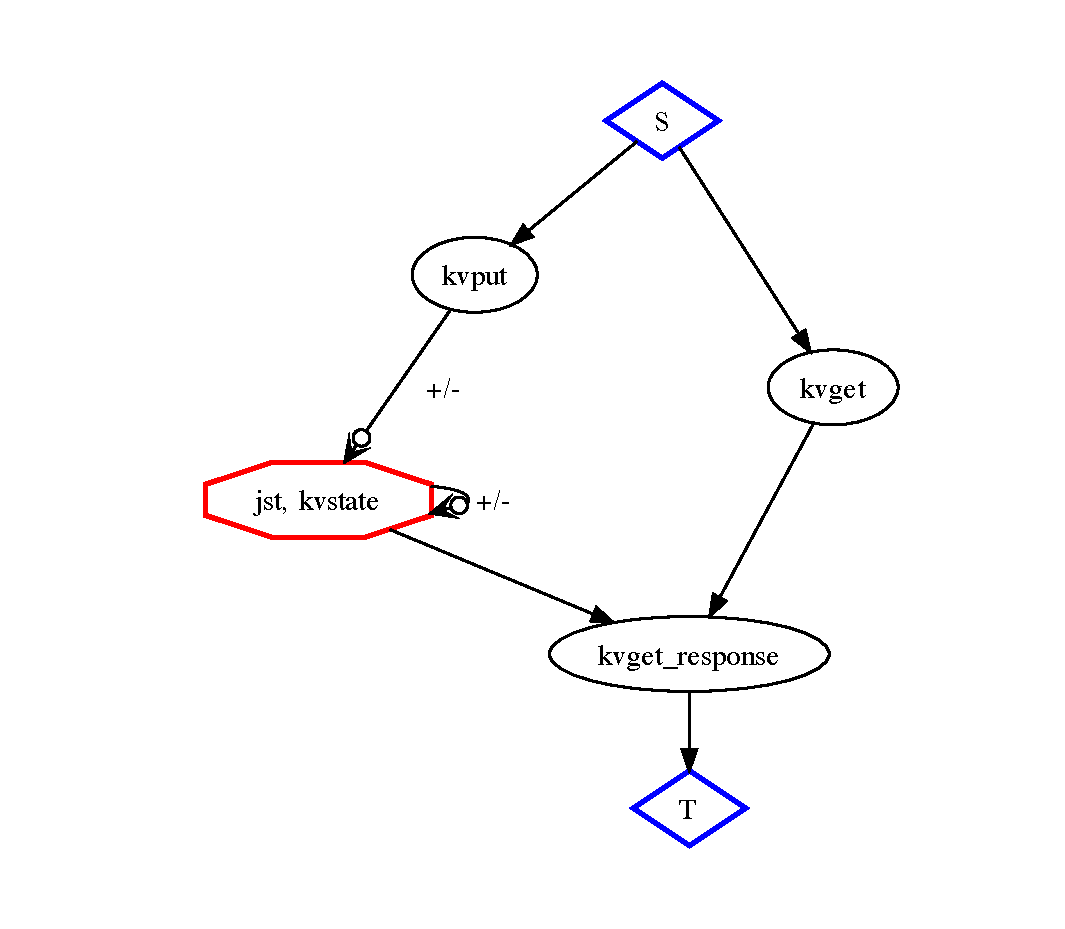
\includegraphics[width=0.55\linewidth]{fig/basickvs.pdf}
\vspace{-10pt}
\caption{Multicast modules.}
\label{fig:multicast-impl}
\end{scriptsize}
\vspace{-2pt}
\end{figure}
